% !TEX root = thesis.tex

\section{El polinomi de Jones}\label{sec:El polinomi de Jones}

El descobriment del \textit{polinomi de Jones} per part de Vaughan Jones l'any 1984 [\cite{jonesoriginal}] dona una manera d'associar a cada nus o link un polinomi de Laurent amb coeficients enters. Aquesta correspondència es fa mitjançant un diagrama de link qualsevol. La teoria de Jones es fonamenta en el fet que si fem un moviment RI, RII o RIII al diagrama del link, aquest polinomi no canvia i doncs és un invariant sota moviments de Reidemeister. El polinomi per un link és doncs independentment del diagrama d'aquest. De manera que si podem veure que dos diagrames de links no tenen el mateix polinomi, llavors segur que aquests son diferents.\\

La manera més simple per definir-lo és mitjançant un altre tipus de polinomi; el \textit{polinomi de Kauffman} descobert per Louis Kauffman.\\

\begin{definition}
	El \underline{polinomi de Kauffman} de $L$, $\langle L\rangle$ és un polinomi de Laurent amb coeficients enters i indeterminada $A$ que podem associar a tot diagrama d'un link a $S^2$ de la següent manera:
	\begin{enumerate}
		\item\label{item:i} $\left\langle\KPA\right\rangle=1$
		\item\label{item:ii} $\left\langle L \cup \KPA\right\rangle=(-A^{-2}-A^{2})\langle L\rangle$
		\item\label{item:iii} $\left\langle\KPB\right\rangle=
		A\left\langle\KPC\right\rangle + A^{-1} \left\langle \KPD \right\rangle$
	\end{enumerate}
\end{definition}

En aquesta definició, $$\KPA$$ és el diagrama del nus zero i $$L \cup \KPA$$ és un diagrama de $L$ juntament amb una corba tancada extra que no conté cap creuament ni amb ella mateixa ni amb $L$. A \textit{\ref{item:iii}} la fórmula relaciona tres diagrames que son el mateix excepte al voltant d'un creuament on es diferencien pels moviments locals indicats. A partir d'aquesta definició és fàcil veure les següents propietats.

\begin{itemize}
	\item $\left\langle\KPA\stackrel{c}{\dots}\KPA\right\rangle=(-A^{-2}-A^{2})^{c-1}$
	\item $\left\langle L\right\rangle=\left\langle rL\right\rangle$
\end{itemize}

La Figura \ref{fig:calculpolinomidekauffman} mostra de forma iterativa el càlcul d'aquest polinomi. Així doncs trobem que $$\left\langle 3_1\right\rangle=A^{-7}-A^{-3}-A^{5}$$ Un exercici similar demostra que $$\left\langle \overline{3_1}\right\rangle=A^{7}-A^{3}-A^{-5}$$

Investiguem ara el comportament del polinomi respecte els moviments de Reidemeister.

\begin{lemma}\label{lem:RI}
	Si a $K$ hi apliquem un moviment RI el seu polinomi de Kauffman canvia de la següent manera $$\left\langle FALTAAAA\right\rangle$$
\end{lemma}

\begin{proof}
	Utilitzant \textit{\ref{item:iii}} i \textit{\ref{item:ii}} en aquest mateix ordre.
\end{proof}

Notem a més que si a \textit{\ref{item:iii}} fessim un moviment local canviant-lo a $$\KPI$$ llavors el polinomi de Kauffman corresponent seria el mateix que l'original intercanviant $A$ per $A^{-1}$. Això significa que si $\overline{K}$ és el nus emmirallat de $K$, llavors $\left\langle\overline{K}\right\rangle=\overline{\left\langle K\right\rangle}$, on $\overline{\left\langle K\right\rangle}$ denota el canvi esmentat anteriorment. Així, observant la Proposició \ref{lem:RI} deduïm que $$FALTA$$ En l'exemple del càlcul del polinomi de Kauffman de $3_1$ anterior també es dona aquest cas.

\begin{figure}
	\centering
	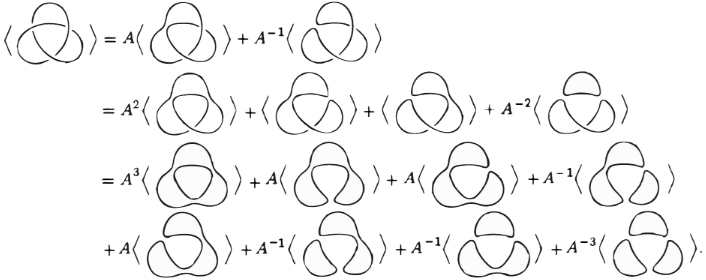
\includegraphics[width=0.9\linewidth]{img/polinomidekauffman.png}
	\caption{Exemple del polinomi de Kauffman de $3_1$.}\label{fig:calculpolinomidekauffman}
\end{figure}

\begin{lemma}\label{lem:RIIiRIII}
	El polinomi de Kauffman és invariant per moviments RII i RIII
\end{lemma}

\begin{proof}
	Per RII cal aplicar \textit{\ref{item:iii}} dues vegades seguides sabent que $\left\langle\overline{K}\right\rangle=\overline{\left\langle K\right\rangle}$ i aplicar-ho en un dels dos creuaments. Per RIII igual.
\end{proof}

\begin{definition}\label{def:torçament}
	Definim el \underline{torçament} $w(L)$ del diagrama d'un link orientat qualsevol com la suma dels signes dels seus creuaments, on cada un d'aquests pren el valor $+1$ o $-1$ com s'indica a la Figura \ref{fig:signe}
\end{definition}

\begin{figure}
	\centering
	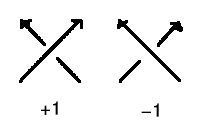
\includegraphics[width=0.9\linewidth]{img/signe.jpg}
	\caption{Signe d'un creuament per la regla de la ma dreta.}\label{fig:signe}
\end{figure}

Notem que la Definició \ref{def:torçament} utilitza la orientació del link. Notem també que aquest és invariant sota moviments RII i RIII i aquest canvia per $+1$ o $-1$ sota moviments RI. La Figura \ref{fig:calculdelsigne} mostra dos exemples sobre el càlcul del torçament d'un nus.\\

\begin{figure}
	\centering
	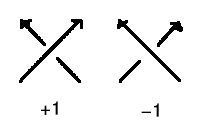
\includegraphics[width=0.9\linewidth]{img/signe.jpg}
	\caption{A l'esquerra el nus $5_1$ que té torçament -5, a la dreta $r5_1$ que té torçament -5.}\label{fig:calculdelsigne}
\end{figure}

El troçament d'un link orientat juntament amb el polinomi de Kauffman d'un diagrama de link sense tenir en compte l'orientació son tots dos invariants sota moviments RII i RIII a més, aquests es comporten d'una manera previsible sota moviments RI. Això duu al següent resultat:

\begin{theorem}
	Sigui $diag(L)$ un diagrama d'un link orientat $L$. Llavors, $$(-A)^{-3w(L)}\left\langle L\right\rangle$$ és un invariant del link orientat $L$.
\end{theorem}

\begin{proof}
	Conseqüència directa del Lema \ref{lem:RIIiRIII}, el Lema \ref{lem:RI} i l'observació sobre el torçament sota moviments $RI$ anterior.
\end{proof}